In this section, we present the clusters of fix patterns that we found in our data set. \RQBC{} is about the borrow-checker related patterns, while \RQG{} is about general patterns. However, our technique fundamentally relies on our data modelling approach successfully capturing the most important aspects of program changes. We thus first evaluate the data modelling approach as our RQ1, before continuing with \RQBC{} and \RQG{}.

\subsection{Evaluating the data modelling approach (RQ1)}

\textbf{Does our data modelling approach capture the most important aspect of program changes?} 

As discussed in the previous section, we used an embedding mechanism to incorporate AST information in fixed-sized datapoints which then could be used in the DBSCAN clustering algorithm. We used heuristics (a weighting scheme) while creating our datapoints to make the most impor tant program elements stand out from all the non terminals seen in the AST (along with some BC-related elements). Here we evaluate the effectiveness of our code embedding.

The general idea for our evaluation is determining whether the most important program elements get high values in our embedding, i.e. are recognized as important. The analyzer compares the actual change in the code and compares it to the visual representation of the respective data point. We used circle pack figures to visualize each data point~\cite{collins2003circle}, generated with the packcircles python library\footnote{\url{https://github.com/mhtchan/packcircles}}. In these figures, the radius of the circle of each non terminal shows its importance in our embedding (as seen in Figure~\ref{fig:essence}).

We collected random samples 1000 times. In each iteration, we collected 50 sample datapoints from our general and borrow-checker databases (25 each). For each database, out of the 1000 sample sets, we picked the one that minimized the sampling error. The sampling error is defined as the absolute difference between the sample mean and the total mean. Also, these random samples are drawn from the clustered datapoints. The reason behind this decision is the same as why we collected a lot of noise points, that is, the majority of the commits contain multi-hunk complex changes and the key changing elements are difficult to determine.

We carried out a manual experiment for evaluating our code embedding. In the experiment, the analyzer should rank the most important element based on the provided circlepack figure and the change's source code. Based on these ranks, then we calculate Top-$n$ Accuracy for $n=1$ up to $n=5$. Both authors carried out the experiment independently. We report the results as the portion of the changes which both authors agreed upon its embedding correctness. The final results are shown in Figure~\ref{fig:rq1}.

\begin{figure}[h]
\centering

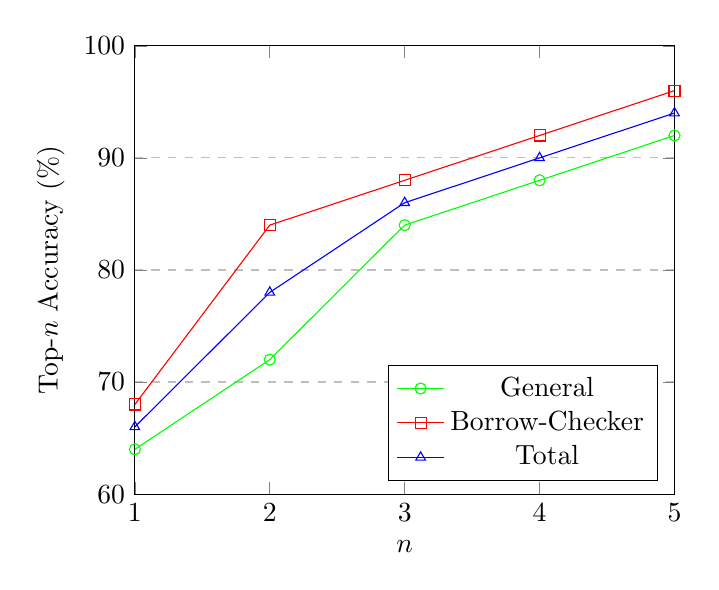
\begin{tikzpicture}
\begin{axis}[
    xlabel={$n$},
    ylabel={Top-$n$ Accuracy (\%)},
    xmin=1, xmax=5,
    ymin=60, ymax=100,
    xtick={1,2,3,4,5},
    ytick={60,70,80,90,100},
    legend pos=south east,
    ymajorgrids=true,
    grid style=dashed,
]

\addplot[
    color=green,
    mark=o,
    ]
    coordinates { 
    (1,64)
    (2,72)
    (3,84)
    (4,88)
    (5,92)
    };
    \addlegendentry{General}

\addplot[
    color=red,
    mark=square,
    ]
    coordinates { 
    (1,68)
    (2,84)
    (3,88)
    (4,92)
    (5,96)
    };
    \addlegendentry{Borrow-Checker}

\addplot[
    color=blue,
    mark=triangle,
    ]
    coordinates { 
    (1,66)
    (2,78)
    (3,86)
    (4,90)
    (5,94)
    };
    \addlegendentry{Total}
    
\end{axis}
\end{tikzpicture}   
\caption{\label{fig:rq1} Top-$n$ Accuracy of the proposed code embedding approach. The plot shows Top-$n$ Accuracy where $n\in\{1,2,3,4,5\}$ for both general and borrow-checker related datapoints. As shown in the plot, in more than 85\% of the datapoints, the most important element is seen at least in the first three ranks.}

\end{figure}

Although, on average, reporting most important element within the top four elements in 90\% of the cases is an accpectable outcome, we examined our pipeline for the other 10\%. The analysis shows that our pipeline fails in change patterns where the change involves many elements (e.g. adding a whole new \verb+impl+ block and implementing new functions in it). It is worth mentioning that these changes tend to be less cross-project as having many changed elements make it easier for datapoints to be dissimlar.

\subsection{\label{sec:common_patterns}Common Bug Fix Patterns (RQ2)}

\textbf{What are the general fix patterns in Rust, and how often do they apply?} 

We collected 60583 datapoints for general fix patterns using a server with a Xeon Gold 5120 processor (Q3-2017, 14-core 2.2 to 3.2GHz) and the data collection took around 26 hours to compute both $D_g$ and $D_b$. We used $\epsilon=0.0001$ and $Z=5$ as our DBSCAN parameters and that resulted in 577 clusters. After manual analysis, as described in~\ref{sec:manual_analysis_cluster_selection}, we ended up with 12 general patterns, which we describe in Table~\ref{table:general}. As it is shown in the table, we have separated the patterns based underlying program element (Category column). We have given each pattern a specific ID (ID column) and determined the number of instances manifesting that fix pattern (\# Instances column), as well as the number of projects in which the pattern was seen (\# Project column). Now we provide detailed description for each of these patterns:

\begin{table}[]

\begin{tabular}{l|l|r|r}
\textbf{Catgegory} & \textbf{ID} & \textbf{\# Instances} & \textbf{\# Projects} \\
\hline
\multirow{2}{*}{Attributes} & G.attr.struct & 172 & 16                                  \\
& G.attr.struct.field & 62 & 16                     \\\cline{1-4}
\multirow{2}{*}{Struct} & G.struct.field  & 179 & 17\\
& G.struct.field.pub & 23 & 12   
\\\cline{1-4}
Option & G.option & 22 & 12                    \\\cline{1-4}
\multirow{4}{*}{Types} & G.type.field  & 72 & 14 \\
& G.type.generic & 46 & 14\\ & G.type.enum.variant  & 39 & 12 \\
& G.type.tuple & 6 & 6                                         \\\cline{1-4}
\multirow{1}{*}{Traits} & G.trait.bound & 6 & 5 \\\cline{1-4}
\multirow{2}{*}{Match} & G.match.pattern & 41 & 12 \\
& G.match.code & 8 & 5 \\
\end{tabular}
\caption{\label{table:general}Bug Fix Pattern Categorization (General Patterns)}
\end{table}
    

\subsubsection{Attributes}

Attributes in Rust enable developers to add metadata to program elements. Developers can add attributes to structs, struct fields, enum variants, match expression arms, etc. There are two types of attributes: Inner Attributes and Outer Attributes. Inner Attributes apply to the program element encapsulating them, while Outer Attributes apply to the program element coming after the attribute. \\

\noindent\textit{\label{sec:G.attr.struct}\textbf{G.attr.struct} Modifying the attributes of structs}

\begin{lstlisting}[language=Rust, style=colouredRust]
// G.attr.struct.add: Adding attributes to a struct
<@\textcolor{green}{++}@> #[derive(Debug, Clone)]
pub struct Call {
/// body 
}

//G.attr.struct.drop: Removing attributes from a struct
<@\textcolor{red}{--}@> #[derive(Debug, Clone)]
pub struct Call {
/// body 
}

// G.attr.struct.change: Changing an existing attribute of a struct
<@\textcolor{red}{--}@> #[derive(Debug)]
<@\textcolor{green}{++}@> #[derive(Debug, Clone)]
pub struct Call {
/// body 
}
\end{lstlisting}

\noindent\textbf{Description:} In this pattern, the attribute set of a struct changes. This modification can happen in three different ways: (G.attr.struct.add) adding attributes to the struct; (G.attr.struct.drop) removing attributes from the struct; and (G.attr.struct.change) changing the content of an existing attribute. These attributes are Outer Attributes as we can find struct related non-terminals within the ASTDiff of the instances of this pattern. \\

\noindent\textit{\textbf{G.attr.struct.field} Modifying the attributes of struct fields}

\begin{lstlisting}[language=Rust, style=colouredRust]
// G.attr.struct.field.add: Adding attributes to struct fields
#[derive(Serialize)]
pub struct Retain {
    <@\textcolor{green}{++}@> #[serde(skip_serializing_if = "is_empty")]
    pub attributes: Option<Attributes>,
}

// G.attr.struct.field.drop: Removing attributes from struct fields
#[derive(Serialize)]
pub struct Retain {
    <@\textcolor{red}{--}@> #[serde(skip_serializing_if = "Option::is_none")]
    pub attributes: Option<Attributes>,
}

// G.attr.struct.field.change: Changing attributes of struct fields
#[derive(Serialize)]
pub struct Retain {
    <@\textcolor{red}{--}@> #[serde(skip_serializing_if = "Option::is_none")]
    <@\textcolor{green}{++}@> #[serde(skip_serializing_if = "is_empty")]
    pub attributes: Option<Attributes>,
}
\end{lstlisting}

\noindent\textbf{Description:} In this pattern, the attribute set of a struct field changes. As with \textit{\textbf{G.attr.struct}}, this modification also happens in three different ways. Using these attributes, the developers can control different actions they wish to apply on struct fields, in addition to providing meta-information.

\subsubsection{Struct} 

Similar to other languages, such as C, a struct makes it possible for the users to define a custom type that is comprised of different types. The patterns that we describe in this section can also be seen in other languages that use the same concept.

\noindent\textit{\textbf{G.struct.field} Adding/Removing a struct field}

\begin{lstlisting}[language=Rust, style=colouredRust]
// G.struct.field.add: Adding a new field to a struct
struct InnerListeners {
    pending: Mutex<Vec<Pending>>,
    <@\textcolor{red}{--}@> queue_object_name: Uuid,
}

// G.struct.field.drop: Removing a field from a struct
struct SnapshotService<U, R> {
    uuid_resolver_handle: R,
    <@\textcolor{green}{++}@> db_name: String,
}
\end{lstlisting}

\noindent\textbf{Description:} A set of new fields are added to or removed from an existing struct. A developer adds a new field to store a new piece of data in a struct. A developer removes a field when the developer realizes that the field is not required with respect to the behaviour they want to implement (possibly because they have moved it elsewhere). \\

\noindent\textit{\textbf{G.struct.field.pub} Modifying the access modifiers of struct fields}

\begin{lstlisting}[language=Rust, style=colouredRust]

// G.struct.field.pub.add: Adding pub to a field
pub struct HtmlBlock {
    <@\textcolor{red}{--}@> content: BlockContent,
    <@\textcolor{green}{++}@> pub content: BlockContent,
    brace: token::Brace,
} 

// G.struct.field.pub.drop: Removing pub from a field
pub struct Languages {
<@\textcolor{red}{--}@>  pub named: HashMap<LanguageId, Arc<LanguageDefinition>>,
<@\textcolor{green}{++}@>  named: HashMap<LanguageId, Arc<LanguageDefinition>>,
    extensions: HashMap<String, Arc<LanguageDefinition>>,
}

\end{lstlisting}

\noindent\textbf{Description:} Adding \texttt{pub} to a struct field makes it possible to access that field from external modules. In the instances of this cluster, adding the \texttt{pub} access modifier happened in a bug fixing change, where the developer needed to access a field which had not been marked for public access. On the other hand, the public access might be revoked if the developer realizes there are no external accesses to the field, and that such accesses are not desirable, e.g. for encapsulation purposes.

\subsubsection{Option}
\vspace{3mm}

\noindent\textit{\textbf{G.option} Changing field type T to T$\langle$Option$\rangle$}

\begin{lstlisting}[language=Rust, style=colouredRust]

#[ast_node("MediaRule")]
pub struct MediaRule {
    pub span: Span,
    <@\textcolor{red}{--}@> pub media: MediaQueryList,
    <@\textcolor{green}{++}@> pub media: Option<MediaQueryList>,
    pub rules: Vec<Rule>,
}

\end{lstlisting}

\noindent\textbf{Description:} Rust is a null-safe language, meaning that object references cannot take on null values. If a developer wants a variable to contain null, they would have to use the \texttt{Option} type. \texttt{Option} is essentially an \texttt{enum} with two variants, \texttt{Some}, which indicates that a variable has a value, and \texttt{None}, which indicates the absence of any value. In this change pattern, the developer changes the type of a struct field to an \texttt{Option} of that type, hence enabling them to store no value in that field.

For instance, in the Rust project swc-project/swc (a fast TypeScript/JavaScript compiler), the developer needed to modify the CSS parser source code to account for empty @media queries\footnote{\scriptsize \url{https://github.com/swc-project/swc/commit/75a14f98b7370226115ee24eec6eb8c802bd4837}}. As shown in the snippet above, they changed type \texttt{MediaQueryList} to \verb+Option<MediaQueryList>+, and modified the other parts of the source code, accordingly.


\subsubsection{Types}

Rust is a statically-typed language, and similar to the other statically-typed languages, some of the change patterns are associated with changes in types used in different program structures. Here, we introduce four bug fix patterns that are associated with types in Rust:

\vspace{3mm}

\noindent\textit{\label{sec:G.type.field}\textbf{G.type.field} Changing a struct field type}

\begin{lstlisting}[language=Rust, style=colouredRust]
pub struct Manifest {
  <@\textcolor{red}{--}@> pub substitutions: HashMap<String, &'a str>,
  <@\textcolor{green}{++}@> pub substitutions: IndexMap<String, &'a str>,
}

\end{lstlisting}

\noindent\textbf{Description:} The type of a struct field changes. This is a common change pattern in all statically-typed languages and can happen for various reasons. For instance, the developer may be implementing a new feature or fixing the behaviour of the program. Also, it can happen for refactoring purposes or performance enhancement. 

For instance, in the Rust project starship/starship (a cross-shell prompt), in order to preserve the insertion order of \verb+substitutions+ field, the developer changes its type from \verb+HashMap+ to \verb+IndexMap+\footnote{\url{https://github.com/starship/starship/commit/4de9e43cff46c834bd340d24a02fc95d85310a33}}.
\\

\noindent\textit{\textbf{G.type.generic} Changing a generic type parameter}

\begin{lstlisting}[language=Rust, style=colouredRust]
#[derive(Debug, Clone, PartialEq)]
pub struct Anchor {
    <@\textcolor{red}{--}@> point: Point<usize>,
    <@\textcolor{green}{++}@> point: Point<isize>,
    side: Side,
}

\end{lstlisting}

\noindent\textbf{Description:} This is a change of the type parameter of a struct field. This change pattern can occur for the same reasons as for \textit{\textbf{G.type.field}}. \\

\noindent\textit{\textbf{G.type.enum.variant} Change in enum variant value type}

\begin{lstlisting}[language=Rust, style=colouredRust]
#[derive(Debug, Clone, PartialEq, Eq)]
pub enum ResolvedDependency {
  Resolved(ModuleSpecifier),
  <@\textcolor{red}{--}@> Err(String),
  <@\textcolor{green}{++}@> Err(ResolvedDependencyErr),
}

\end{lstlisting}

\noindent\textbf{Description:} In Rust, developers can specify the type of the value that an enum variant can store. Using this feature, they can avoid having to use a struct along with enum variants. This change pattern is associated with a change in enum variant types. \\


\noindent\textit{\textbf{G.type.tuple} Changing the type inside a tuple}

\begin{lstlisting}[language=Rust, style=colouredRust]
#[allow(dead_code)]
pub struct CoreState {
    // Other fields
    <@\textcolor{red}{--}@> pending_views: Vec<ViewId>,
    <@\textcolor{green}{++}@> pending_views: Vec<(ViewId, Table)>,
    peer: Client
}
\end{lstlisting}



\noindent\textbf{Description:} In this pattern, an extra type is added to an existing type, making it a tuple of multiple types. Alternatively, the change might be dropping types from the tuple and making it a smaller-arity tuple.

\subsubsection{Traits}
\noindent\textit{\textbf{G.trait.bound} TraitBound change}

\begin{lstlisting}[language=Rust, style=colouredRust]
<@\textcolor{red}{--}@> pub struct EventLoop<T: tty::EventedReadWrite> {
<@\textcolor{green}{++}@> pub struct EventLoop<T: tty::EventedPty> {
    poll: mio::Poll,
    // Other fields
}

\end{lstlisting}

\noindent\textbf{Description:} The trait bounds are the functionalities that we require from our parametric types. This concept might be referred to as interfaces in other languages, although there might be small differences. This change pattern relates to modifications in trait bounds. This can happen as part of bug fixes or for refactoring. \\

\subsubsection{Match}

In Rust, match control flow construct is used for comparing a value against multiple patterns, and executing the code associated with the first pattern that matches with our value. A pattern and its associated code are called a match arm. Match statements can be similar to switch statements in other languages, like C, although match statements in Rust are able to match more complicated patterns.\\

\noindent\textit{\textbf{G.match.pattern} Change in a match arm's pattern}

\begin{lstlisting}[language=Rust, style=colouredRust]
<@\textcolor{red}{--}@> Value::Primitive(p) => {
<@\textcolor{green}{++}@> UntaggedValue::Primitive(p) => {
    let _ = builder.add_empty_child(p.format(None));
}
\end{lstlisting}

\noindent\textbf{Description:} In this pattern, a change occurs in an arm's pattern. Like the code snippet provided above, it can be a change in pattern's type. It also can be matching to a different enum variant or string. The fix pattern can happen both for refactoring or debugging purposes. \\

\noindent\textit{\textbf{G.match.code} Change in a match arm's code}

\begin{lstlisting}[language=Rust, style=colouredRust]
Operation::Insert(insert) => {
    <@\textcolor{red}{--}@> inverted.delete(insert.count_of_utf16_code_units());
    <@\textcolor{green}{++}@> inverted.delete(insert.utf16_size());
}
\end{lstlisting}

\noindent\textbf{Description:} The block of code associated with a pattern in match arm can contain multiple statements. In this fix pattern, a change happens in at least one of these statements. Similar to the previous fix pattern, this also can be due to refactoring or debugging purposes.

\subsection{\label{sec:bc_patterns}BC-Related Bug Fix Patterns (RQ3)}

\textbf{What are borrow-checker related fix patterns in Rust, and how often do they apply?} 

We collected 27143 datapoints for borrow-checker related fix patterns. We used $\epsilon=0.001$ and $Z=5$ as our DBSCAN parameters and that resulted in 102 clusters. After manual analysis, as described in~\ref{sec:manual_analysis_cluster_selection}, we ended up with 8 borrow-checker related fix patterns, which we, similar to the previous table, describe in Table~\ref{table:bc}. Here we provide detailed description for each of these patterns:

\begin{table}[]
\begin{tabular}{l|l|r|r}
\textbf{Catgegory} & \textbf{ID} & \textbf{\# Instances} & \textbf{\# Projects} \\
\hline
\multirow{2}{*}{Clone}                                         & BC.clone.drop & 83 & 10 \\
& BC.clone.ref & 4 & 3   
\\\cline{1-4}
\multirow{2}{*}{Ref and Deref} & BC.ref.add & 17 & 7 \\
& BC.deref.to\_string.add  & 4 & 3                                            \\\cline{1-4}
\multirow{2}{*}{Mut} & BC.mut.add  & 11 & 6 \\
& BC.mut.drop  & 42 & 15                               \\\cline{1-4}
Vector & BC.vec.slice  & 8 & 6                                    \\\cline{1-4}
\multirow{1}{*}{Lifetime}      
& BC.lifetime.static  & 8 & 6
\\
\end{tabular}
\caption{\label{table:bc}Bug Fix Pattern Categorization (BC-Related Patterns)}
\end{table}
    

\subsubsection{Clone}

\noindent\textit{\textbf{BC.clone.drop} Dropping clone}

\begin{lstlisting}[language=Rust, style=colouredRust]
start_plugin_process(
<@\textcolor{red}{--}@>  manifest.clone(),
<@\textcolor{green}{++}@>  manifest,
    self.next_plugin_id(),
    self.self_ref.as_ref().unwrap().clone(),
);
\end{lstlisting}

\noindent\textbf{Description:} This pattern is referred to as redundant clone in Clippy Lints. Clippy\footnote{\url{https://github.com/rust-lang/rust-clippy}} is a linter tool for Rust that catches common mistakes. There are more than 500 lints included in Clippy. With regards to this pattern, Clippy detects whether a variable clone is necessary, i.e. could the developer have used the variable itself or not. It is evident that removing a redundant clone does not modify the program behaviour, however it can boost the performance significantly if the program was repeatedly cloning large variables. \\

\noindent\textit{\textbf{BC.clone.ref} Dropping clone and adding borrowing}

\begin{lstlisting}[language=Rust, style=colouredRust]
<@\textcolor{red}{--}@> let field_id = schema.get_or_create(attribute.clone())?;
<@\textcolor{green}{++}@> let field_id = schema.get_or_create(&attribute)?;
\end{lstlisting}

\noindent\textbf{Description:} Unlike the previous pattern, this pattern is not detected by Clippy. The change happens when a developer realizes that the cloning of a variable is unnecessary, but also wants to keep the ownership of the variable within the current scope (rather than passing it to a callee). That is why, in this pattern, a clone is turned into a borrow. 

Like the previous pattern, this change does not affect the program behaviour; it is done for performance purposes. In one of the commits\footnote{\scriptsize \url{https://github.com/tauri-apps/tauri/commit/a280ee90af0749ce18d6d0b00939b06473717bc9}} of the project tauri-apps/tauri, changing a clone to borrowing significantly improved CPU usage. In the commit history, developers discussed how the cloning of types such as HashMap was expensive. \\

\subsubsection{Ref and Deref}

\noindent\textit{\textbf{BC.ref.add} Adding Borrowing}

\begin{lstlisting}[language=Rust, style=colouredRust]
let repo = replace(&mut *contents, Processing).inner_repo();
<@\textcolor{red}{--}@> let statuses = repo_to_statuses(repo, &self.workdir);
<@\textcolor{green}{++}@> let statuses = repo_to_statuses(&repo, &self.workdir);
\end{lstlisting}

\noindent\textbf{Description:} This change pattern happens when the developer now needs to take back ownership of an object that was previously passed to a callee (or other scope) and never returned. Borrowing allows the first scope to once again act on the object.

To give an example, the commit in starship/starship excerpted above\footnote{\scriptsize \url{https://github.com/starship/starship/commit/56d475578ea508631275772127f49a6949fea6b0}} shows that the developer now borrows the value of \verb+repo_dir+ to keep the ownership of the object in the current scope. This object can then be used in a subsequent function invocation (\verb+remove_dir_all(repo_dir)+), which fixes a bug. \\

\noindent\textit{\textbf{BC.deref.to\_string().add} Adding a dereference operation before calling to\_string()}

\begin{lstlisting}[language=Rust, style=colouredRust]
for p in wixobjs {
<@\textcolor{red}{--}@>  args.push(p.to_string());
<@\textcolor{green}{++}@>  args.push((*p).to_string());
}

\end{lstlisting}

\noindent\textbf{Description:} This is a change that in all instances has been detected by Clippy (commit messages indicated the use of Clippy for this fix). The change applies on an object prior to calling \verb+to_string()+ on that object. The change might add or remove a dereference, as shown above. When adding a dereference, the reason behind the change is that the object is a reference type of \verb+T+, while \verb+T+ directly implements \verb+to_string()+. Adding the dereference makes the compiler use the specialized implementation of \verb+to_string()+ and not go through slower string formatting methods.


\subsubsection{Mut}

\noindent\textit{\textbf{BC.mut.add} Adding mutability}

\begin{lstlisting}[language=Rust, style=colouredRust]
parser::Parser::new(args)
        .parse_module()
<@\textcolor{red}{--}@>      .map_err(|e| {
<@\textcolor{green}{++}@>      .map_err(|mut e| {
            e.emit();
            ()
        })?
\end{lstlisting}

\noindent\textbf{Description:} This change happens when the developer needs to mutate a variable which was previously immutable in a scope---they thus need to add the mut keyword. We never observed this pattern in refactoring changes; it always accompanied a change in program behaviour. \\

\noindent\textit{\textbf{BC.mut.drop} Dropping mutability}

\begin{lstlisting}[language=Rust, style=colouredRust]
<@\textcolor{red}{--}@> let mut tx = tx.clone();
<@\textcolor{green}{++}@> let tx = tx.clone();
\end{lstlisting}

\noindent\textbf{Description:} The developer drops the mut keyword before a variable, as they do not mutate the variable. This redundant mutability is reported by Clippy and can also be removed by it. This change may help future-proof the code against unintended future changes.

\subsubsection{Vector}

\noindent\textit{\textbf{BC.vec.slice} Changing a Vec reference to Slice}

\begin{lstlisting}[language=Rust, style=colouredRust]
pub fn expand_delimited_square(
<@\textcolor{red}{--}@>  children: &Vec<TokenNode>,
<@\textcolor{green}{++}@>  children: &[TokenNode],
) -> Result<hir::Expression, ParseError> {
    // body
}
\end{lstlisting}
\noindent\textbf{Description:} In a struct field definition, or in the types of a function's formal parameters, type \verb+&Vec<T>+ changes to slice \verb+&[T]+. Clippy can detect the opportunity to apply this pattern. This simplifies the code; slice types \verb+&[T]+ or \verb+&str+ are sufficient for most use cases. 

\subsubsection{Lifetime}
\noindent\textit{\textbf{BC.lifetime.static.drop} Dropping static lifetime}

\begin{lstlisting}[language=Rust, style=colouredRust]
<@\textcolor{red}{--}@> const QUEUE_SIZES: &'static [u16] = &[QUEUE_SIZE];
<@\textcolor{green}{++}@> const QUEUE_SIZES: &[u16] = &[QUEUE_SIZE];

\end{lstlisting}

\noindent\textbf{Description:} This change pattern removes the static keyword from a const variable declaration. This change can be applied using Clippy. If the presence of static is not required, it is better that to omit it, as keeping it might create complicated types in the program.

